
%! program = pdflatex

\documentclass[12pt]{article}
\usepackage{amsmath}
\usepackage{natbib}
\usepackage{graphicx}
\usepackage{amssymb}
\usepackage{epstopdf}
\usepackage{float} % to keep the figures in place

\usepackage{color}
\newcommand{\cred}{ \color{red}}
\newcommand{\cgreen}{\color{green}}
\newcommand{\cblue}{\color{blue}}
\newcommand{\cmag}{\color{magenta}}
\newcommand{\bn}{\begin{enumerate}}
\newcommand{\en}{\end{enumerate}}
\newcommand{\bi}{\begin{itemize}}
\newcommand{\ei}{\end{itemize}}
\newcommand{\be}{\begin{eqnarray}}
\newcommand{\ee}{\end{eqnarray}}
\newcommand{\by}{\begin{eqnarray*}}
\newcommand{\ey}{\end{eqnarray*}}
\renewcommand{\labelenumi}{(\alph{enumi}) }
%
\usepackage[margin=2.2cm, includehead]{geometry}% see geometry.pdf on how to lay out the page. There's lots.
\geometry{letterpaper} % or letter or a5paper or ... etc
% \geometry{landscape} % rotated page geometry
%\bibpunct{(}{)}{;}{a}{,}{,}
%\setlength{\textwidth}{16cm}
%\setlength{\textheight}{21cm}
\def\nonumber{\global\@eqnswfalse}
\newcounter{parnum}
\newcommand{\N}{%
  \noindent\refstepcounter{parnum}%
   \makebox[\parindent][l]{\textbf{[\arabic{parnum}]}}\quad  }
% Use a generous paragraph indent so numbers can be fit inside the
% indentation space.
\setlength{\parindent}{1.5em}

% See the ``Article customise'' template for come common customisations

\date{}
%\date{} % delete this line to display the current date

%%% BEGIN DOCUMENT
\usepackage{Sweave}
\begin{document}
\Sconcordance{concordance:HW6.tex:HW6.Rnw:%
1 47 1 1 0 21 1 1 18 4 0 1 1 3 0 1 1 3 0 1 1 3 0 1 1 1 2 5 1 1 3 1 2 4 %
1 1 4 1 2 7 1 1 2 4 0 1 2 1 1 1 3 2 0 1 2 1 0 2 1 1 6 5 0 1 1 6 0 1 2 3 %
1 1 2 1 0 3 1 4 0 1 2 4 1 1 2 1 0 4 1 1 6 5 0 1 1 1 6 5 0 1 1 5 0 1 1 6 %
0 1 2 3 1 1 2 1 0 2 1 4 0 1 2 5 1 1 2 1 0 2 1 4 0 1 2 8 1 1 3 1 2 4 1 1 %
6 1 2 4 1 1 4 1 2 3 1 1 2 4 0 1 2 1 1 1 3 2 0 2 1 1 6 5 0 1 1 6 0 1 2 2 %
1 1 2 1 0 3 1 4 0 1 2 5 1 1 2 1 0 4 1 1 6 5 0 1 1 1 6 5 0 1 1 5 0 1 1 6 %
0 1 2 3 1 1 2 1 0 2 1 4 0 1 2 5 1 1 2 1 0 2 1 4 0 1 2 9 1 1 3 1 2 1 1 1 %
2 4 0 1 2 1 1 1 3 2 0 2 1 1 6 5 0 1 1 6 0 1 2 2 1 1 2 1 0 3 1 4 0 1 2 4 %
1 1 2 1 0 4 1 1 6 5 0 1 1 1 6 5 0 1 1 5 0 1 1 6 0 1 2 3 1 1 2 1 0 2 1 4 %
0 1 2 5 1 1 2 1 0 2 1 4 0 1 2 9 1 1 6 1 2 2 1 1 2 5 0 1 2 4 1 1 3 1 2 4 %
1 1 4 1 2 8 1 1 2 1 0 1 1 7 0 1 2 3 1 1 2 1 0 1 1 7 0 1 2 3 1 1 2 1 0 1 %
1 7 0 1 2 3 1 1 2 1 0 1 1 7 0 1 2 3 1}

%\large
%\maketitle
\newtheorem{thm}{Theorem}[section]
\newtheorem{cor}[thm]{Corollary}
\newtheorem{lem}[thm]{Lemma}
\newtheorem{prop}[thm]{Proposition}
\newtheorem{defn}[thm]{Definition}
\newtheorem{exam}[thm]{Example}
\newtheorem{qstn}[thm]{Question}

%%%
\newpage
\begin{center}
{\bf Homework 6 - STAT 511}\\
Amal Agarwal
\end{center}
%==========================
\section*{Answer 3}
\bn
\item The estimated parameters obtained by fitting the pairs $(x_i,y_i)$ for $i=1,2,3,4$ are respectively given as
\begin{Schunk}
\begin{Soutput}
(Intercept)          x1 
  3.0000909   0.5000909 
\end{Soutput}
\begin{Soutput}
(Intercept)          x2 
   3.000909    0.500000 
\end{Soutput}
\begin{Soutput}
(Intercept)          x3 
  3.0024545   0.4997273 
\end{Soutput}
\begin{Soutput}
(Intercept)          x4 
  3.0017273   0.4999091 
\end{Soutput}
\end{Schunk}

\item
\begin{itemize}
\item Analysis of $(x_1, y_1)$ within the linear model framework:\\
Scatter plot of $(x_1, y_1)$ along the fitted line is given as:
\begin{figure}[H]
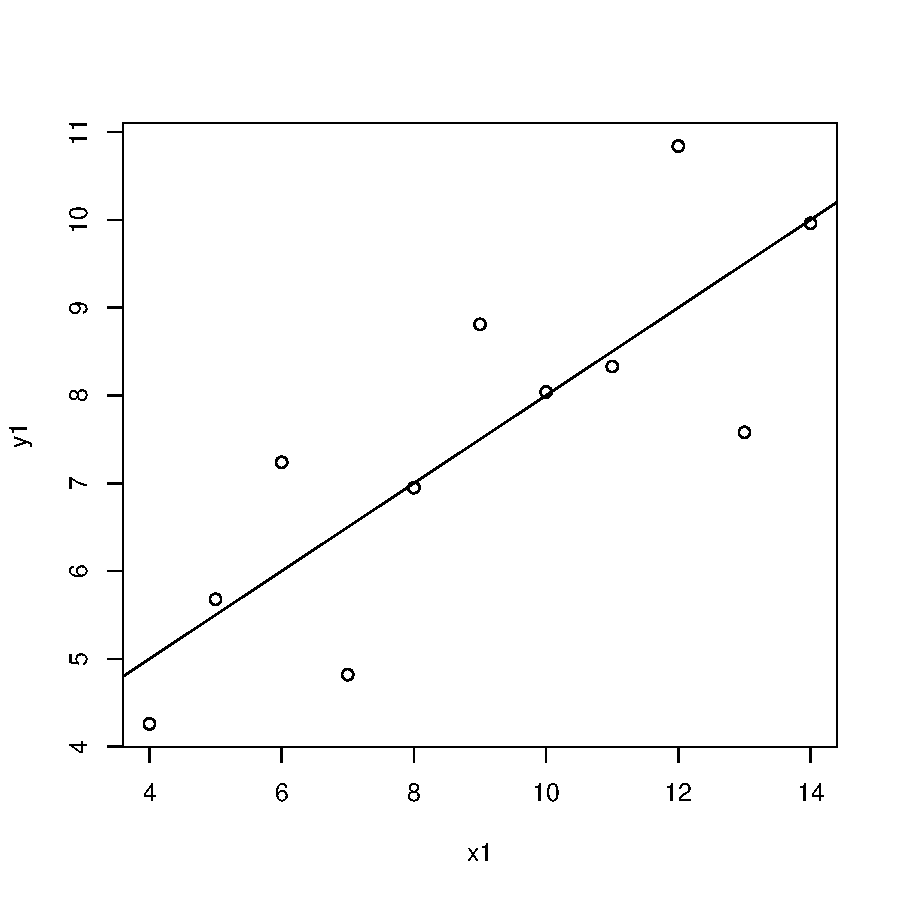
\includegraphics{HW6-002}
\end{figure}
The relationship looks linear from the scatter plot.\\
\clearpage
The residual plot is given as
\begin{figure}[H]
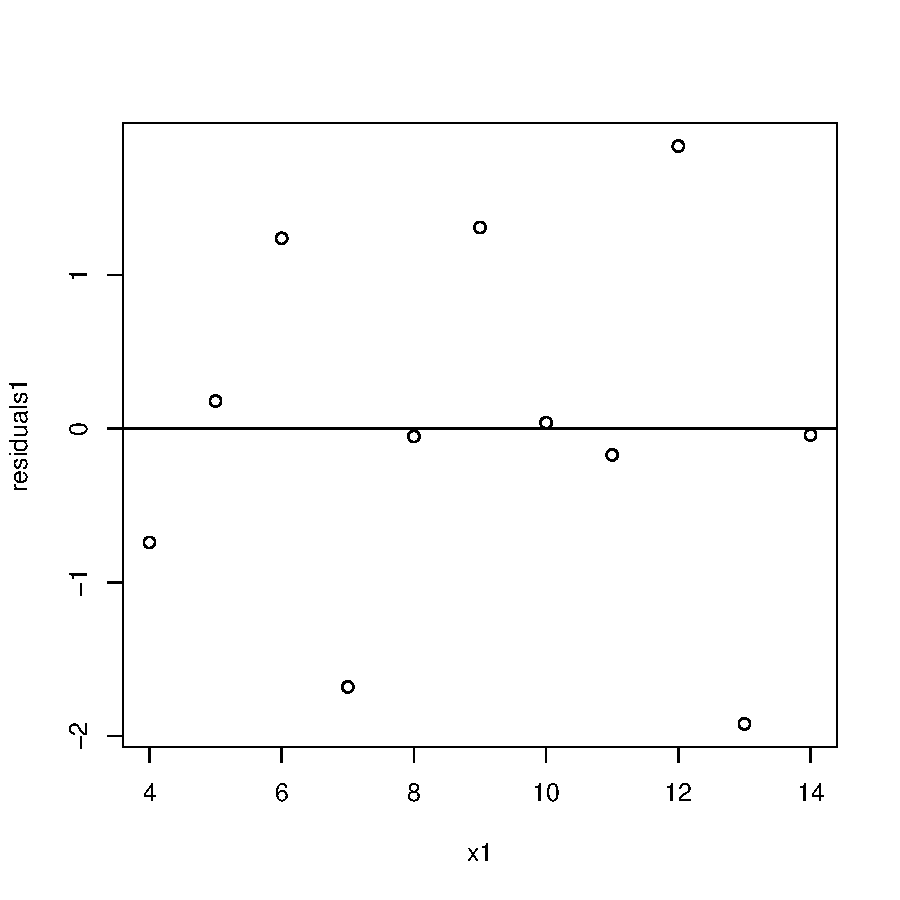
\includegraphics{HW6-003}
\end{figure}
The above residual plot shows that the residuals are almost uniformly distributed around 0. Thus our assumption of homoscedascity is verified. There is no positive or negative correlation between successive values of residuals which verifies the assumption of independence. Further there is no identifiable non-linear trend and thus we can also say that our assumption of linearity is verified.\\

To check for possible outliers, we can do a leave one out analysis to get the studentized residuals and construct the following test.\\

$H_0$: Linear Model is correctly specified.\\
Reject $H_0$ if $r_{0}^{*}>t\left((1-\dfrac{\alpha}{2}),(n-p-1)\right)$ where $t\left((1-\dfrac{\alpha}{2}),(n-p-1)\right)$ is the $(1-\dfrac{\alpha}{2})$ quantile of a t-distribution with $(n-p-1)$ degrees of freedom. This follows from the fact that $r_{i}^{*}=\dfrac{\widehat{\epsilon_{(i)}}}{\widehat{\sigma_{(i)}}\left(\sqrt{1+\underline{X_{i}^{'}}(X_{(i)}^{'}X_{(i)})^{-1}\underline{X_{i}}}\right)}$ follows a t-distribution with $(n-p-1)$ degrees of freedom. The studentized residuals are calculated as:

\begin{Schunk}
\begin{Sinput}
> rst1<-rstudent(fit1)
\end{Sinput}
\end{Schunk}
The following R code compares the values of the studentized residuals with the $\left(1-\dfrac{\alpha}{2}\right)$ quantile values of the t-distribution.

\begin{Schunk}
\begin{Sinput}
> # level of significance
> alpha<-0.05
> # observation numbers of the outliers
> out1<-rep(0,length(x1))
> rst1<-rstudent(fit1)
> j=1
> for (i in 1:length(x1)){
+   if (rst1[i]>qt((1-(alpha/(2*length(x1)))),(n-p-1))){
+     out1[j]<-i
+     j<-j+1
+   }
+ }
> out1
\end{Sinput}
\begin{Soutput}
 [1] 0 0 0 0 0 0 0 0 0 0 0
\end{Soutput}
\end{Schunk}
\clearpage

Plotting the studentized residuals
\begin{figure}[H]
\begin{Schunk}
\begin{Sinput}
> plot(rst1)
> cutoff=qt(.975,df=n-p-1)
> abline(h=cutoff)
> abline(h=-cutoff)
\end{Sinput}
\end{Schunk}
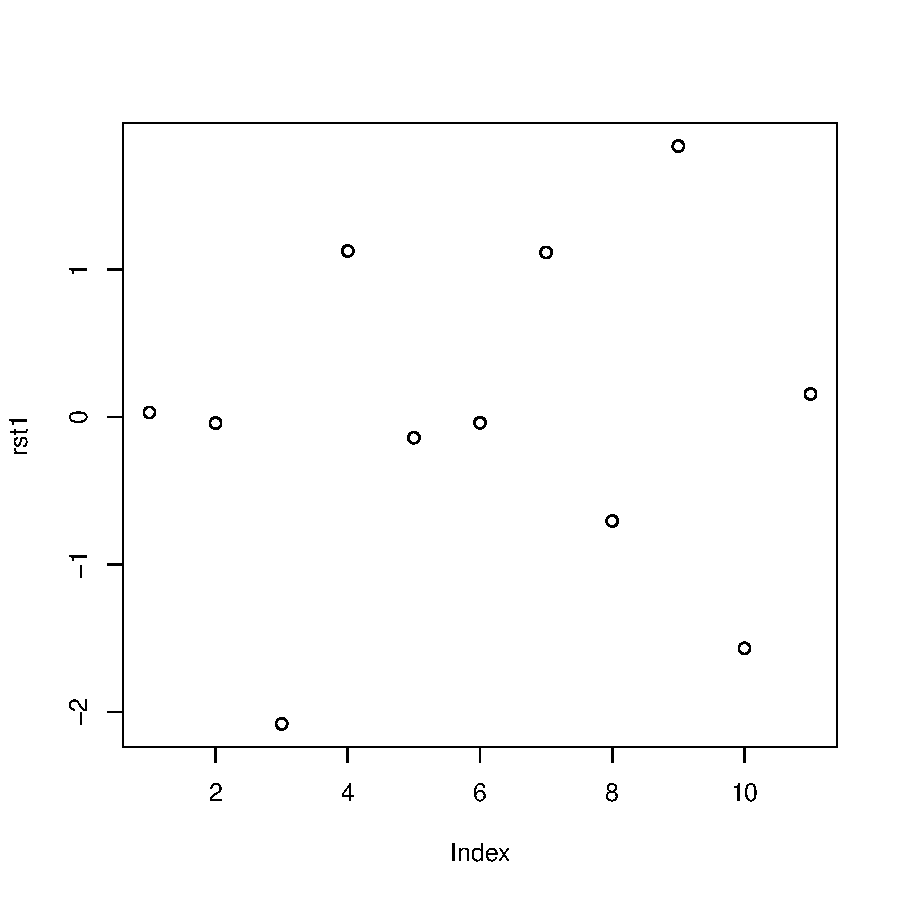
\includegraphics{HW6-006}
\end{figure}

In the above plot, the cutoff lines go out of the bounds. Therefore there are no outliers and hence our null hypothesis is not rejected.\\
The influential points can be found by looking at various diagnostic measures like leverage i.e. diagonal elements of Hat matrix ($h_{ii}$) and Cook's distance (CD). We consider an observation likely to be influential if $h_{ii}>\dfrac{2p}{n}$ or $CD_{i}>1$. This is done using the following R code:

\begin{Schunk}
\begin{Sinput}
> hii1<-hatvalues(fit1)
> cd1<-cooks.distance(fit1)
> inf1.1<-rep(0,length(x1))
> inf1.2<-rep(0,length(x1))
> j=1
> for (i in 1:length(x1)){
+   if (hii1[i]>(2*p/n)){
+     inf1.1[j]<-i
+     j<-j+1
+   }
+ }
> j=1
> for (i in 1:length(x1)){
+   if (cd1[i]>1){
+     inf1.2[j]<-i
+     j<-j+1
+   }
+ }
> inf1.1
\end{Sinput}
\begin{Soutput}
 [1] 0 0 0 0 0 0 0 0 0 0 0
\end{Soutput}
\begin{Sinput}
> inf1.2
\end{Sinput}
\begin{Soutput}
 [1] 0 0 0 0 0 0 0 0 0 0 0
\end{Soutput}
\end{Schunk}
\clearpage

Plotting the diagonal hat values:
\begin{figure}[H]
\begin{Schunk}
\begin{Sinput}
> cutoff.h<-2*p/n
> plot(hii1)
> abline(h=cutoff.h)
\end{Sinput}
\end{Schunk}
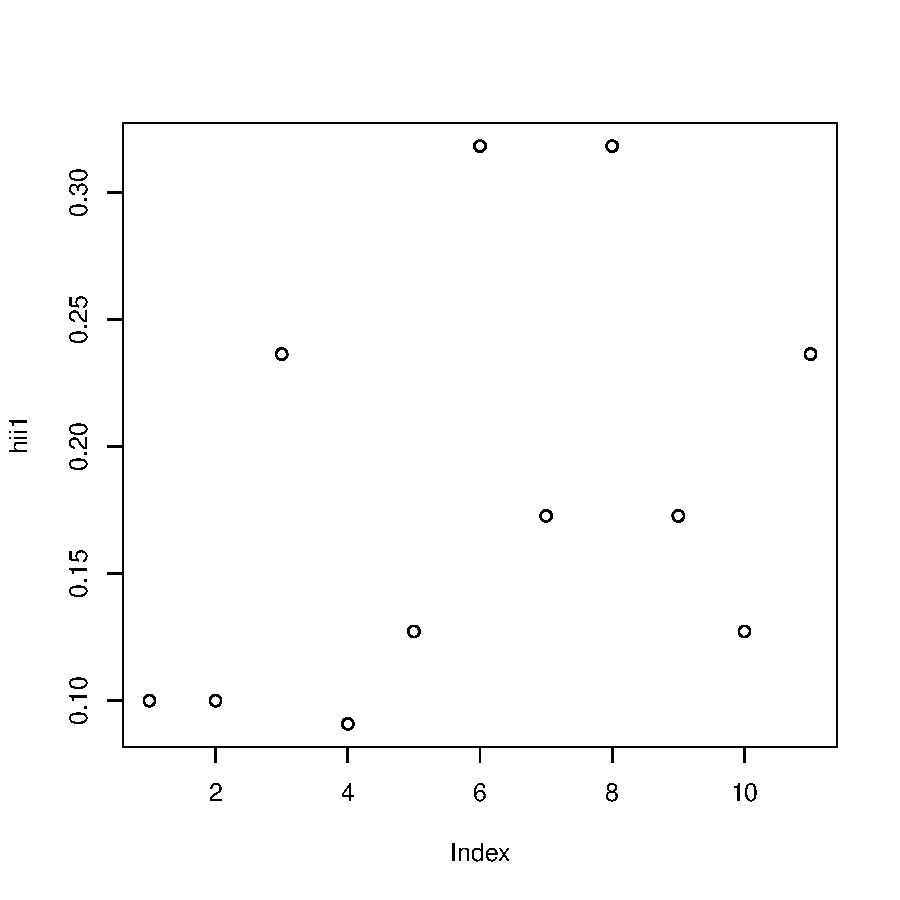
\includegraphics{HW6-008}
\end{figure}
Again the cutoff line in the above graph is out of the bounds.
\clearpage

Plot of Cook's distance values:
\begin{figure}[H]
\begin{Schunk}
\begin{Sinput}
> cutoff.cd1<-1
> plot(cd1)
> abline(h=cutoff.cd1)
\end{Sinput}
\end{Schunk}
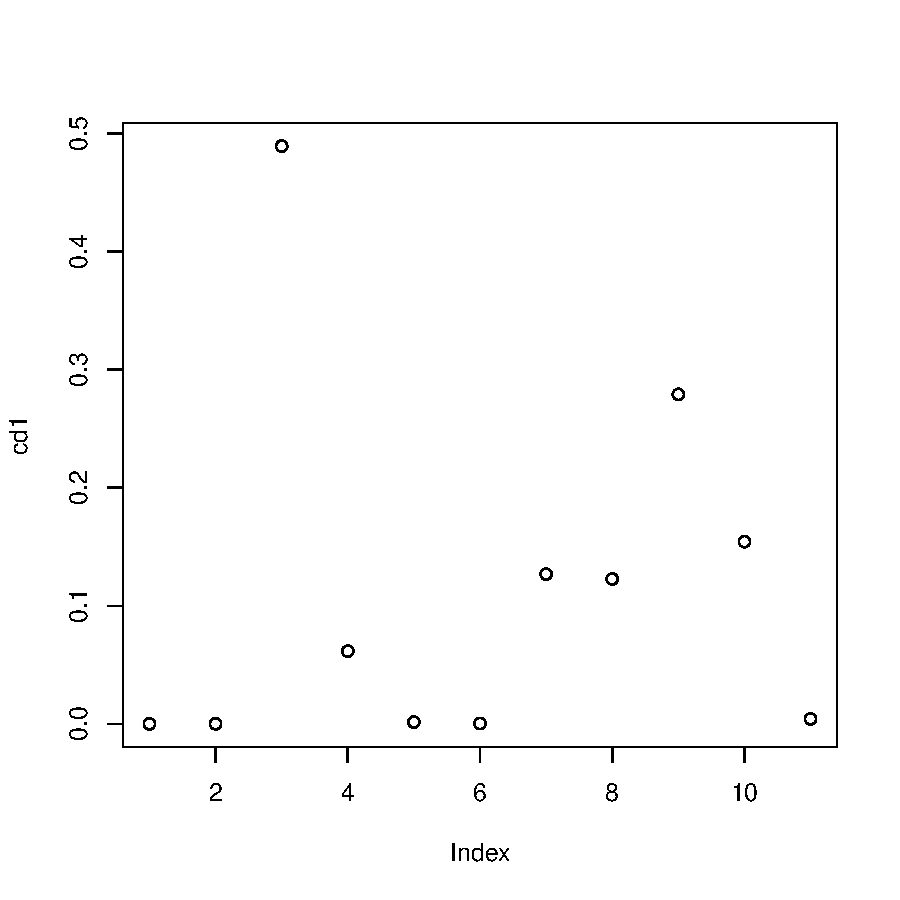
\includegraphics{HW6-009}
\end{figure}
Again the cutoff line in the above graph is out of the bounds.

Thus we find no influential points with both the leverage criterion and the Cook's distance criterion.
\clearpage

\item Analysis of $(x_2, y_2)$ within the linear model framework:\\
Scatter plot of $(x_2, y_2)$ along the fitted line is given as:
\begin{figure}[H]
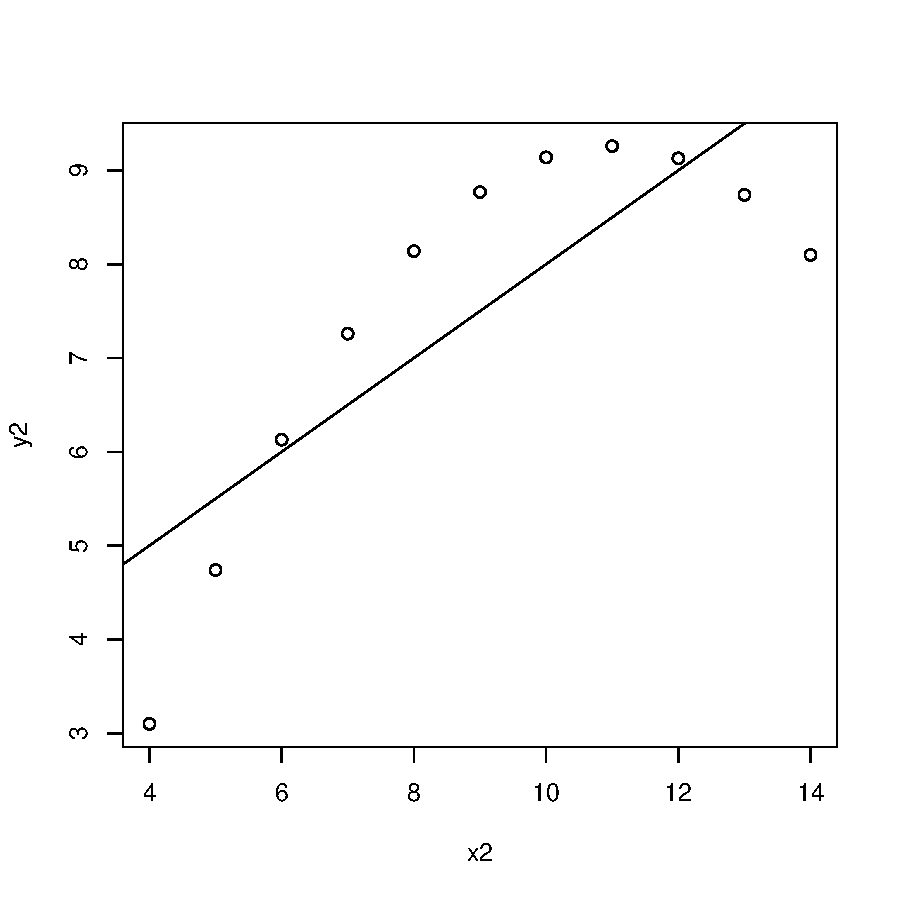
\includegraphics{HW6-010}
\end{figure}
This scatter plot shows a non-linear relationship between the response and predictor. It likes look y depends on x quadratically.\\

Fitting a polynomial of degree 2 in x2, we obtain the following scatter plot along with the fitted line
\begin{figure}[H]
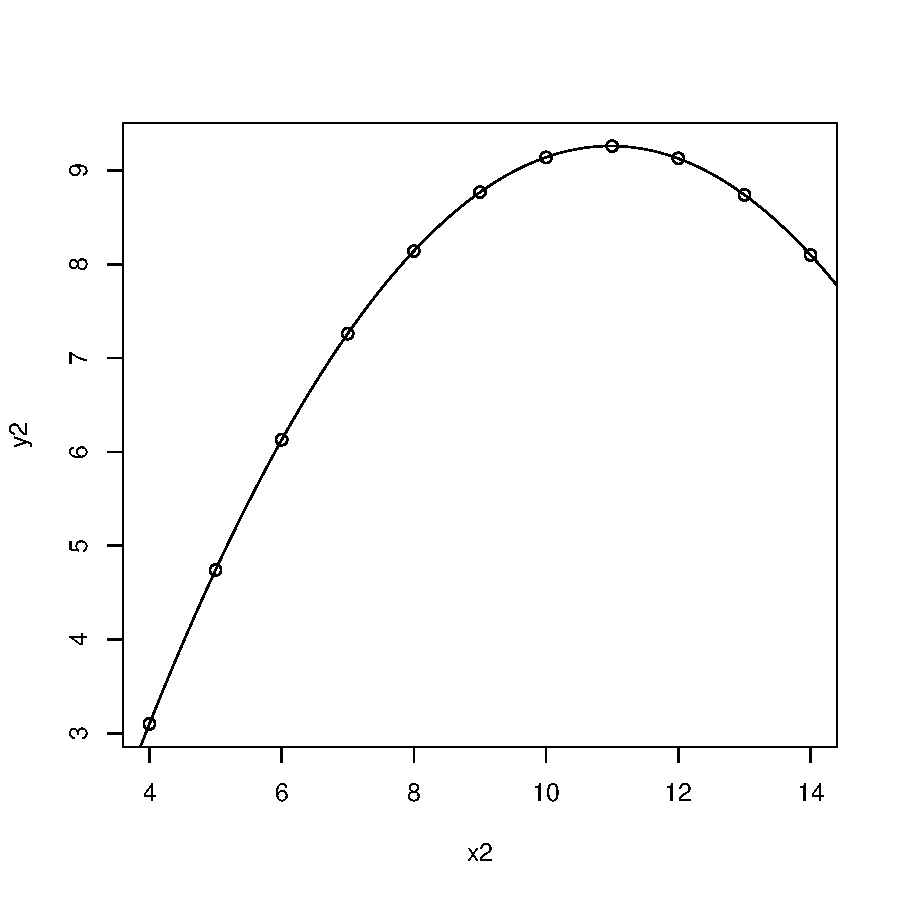
\includegraphics{HW6-011}
\end{figure}

\clearpage
The residual plot is given as
\begin{figure}[H]
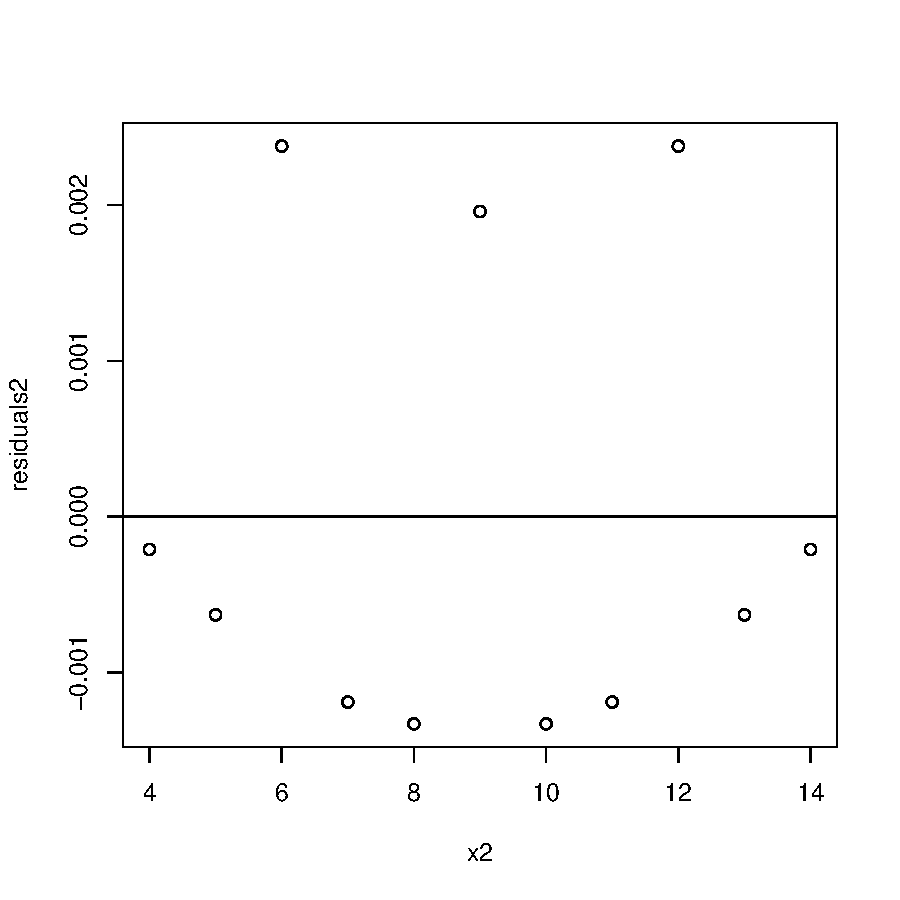
\includegraphics{HW6-012}
\end{figure}
The above residual plot shows that the residuals are not uniformly distributed around 0. Thus our assumption of homoscedascity is violated. But still there does not seem any positive or negative correlation between successive values of residuals which verifies the assumption of independence. Clearly there is a non-linear trend that has been taken into account already by using polynomial transformation of degree 2.\\

To check for possible outliers, we calculate the studentized residuals and do the test as before:
\begin{Schunk}
\begin{Sinput}
> rst2<-rstudent(fit2.2)
\end{Sinput}
\end{Schunk}
The following R code compares the values of the studentized residuals with the $\left(1-\dfrac{\alpha}{2}\right)$ quantile values of the t-distribution.

\begin{Schunk}
\begin{Sinput}
> # observation numbers of the outliers
> out2<-rep(0,length(x2))
> rst2<-rstudent(fit2.2)
> j=1
> for (i in 1:length(x2)){
+   if (rst2[i]>qt((1-(alpha/(2*length(x2)))),(n-p-1))){
+     out2[j]<-i
+     j<-j+1
+   }
+ }
> out2
\end{Sinput}
\begin{Soutput}
 [1] 0 0 0 0 0 0 0 0 0 0 0
\end{Soutput}
\end{Schunk}

Plotting the studentized residuals:
\begin{figure}[H]
\begin{Schunk}
\begin{Sinput}
> plot(rst2)
> cutoff<-qt(.975,df=n-p-1)
> abline(h=cutoff)
> abline(h=-cutoff)
\end{Sinput}
\end{Schunk}
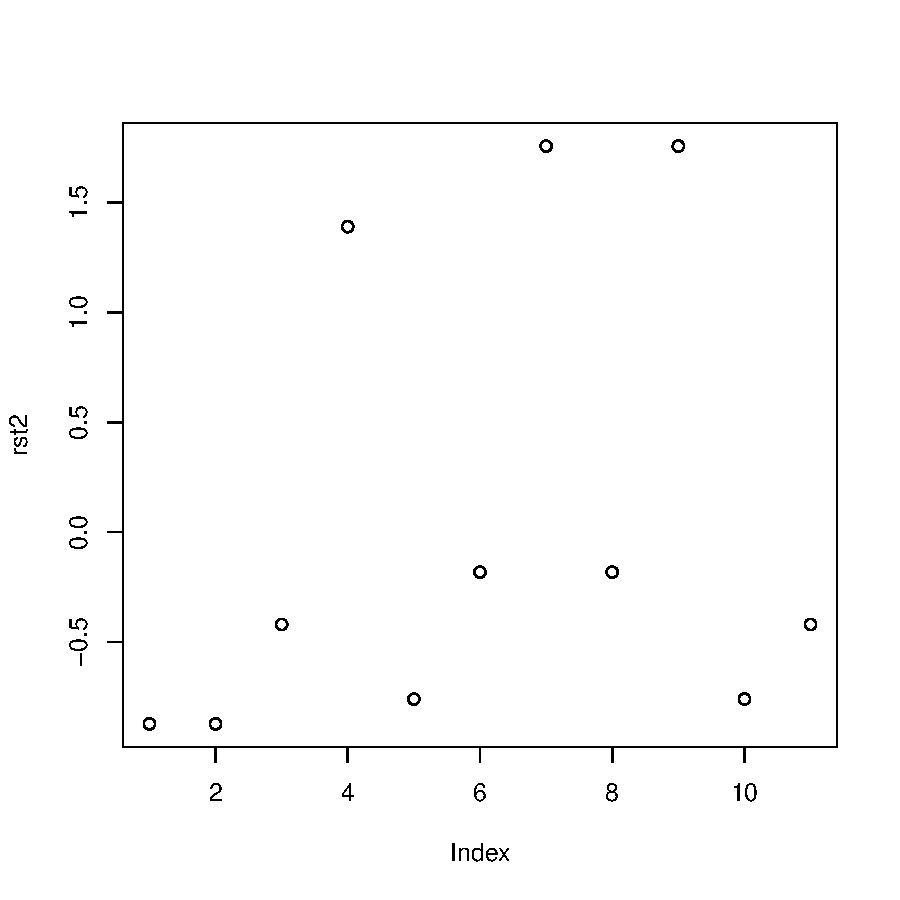
\includegraphics{HW6-015}
\end{figure}

In the above plot, the cutoff lines go out of the bounds. Therefore there are no outliers and hence our null hypothesis is not rejected.\\

Again influential points were found using the leverage and Cook's distance criteria as follows:

\begin{Schunk}
\begin{Sinput}
> hii2<-hatvalues(fit2.2)
> cd2<-cooks.distance(fit2.2)
> inf2.1<-rep(0,length(x2))
> inf2.2<-rep(0,length(x2))
> j=1
> for (i in 1:length(x2)){
+   if (hii2[i]>(2*p/n)){
+     inf2.1[j]<-i
+     j<-j+1
+   }
+ }
> j=1
> for (i in 1:length(x2)){
+   if (cd2[i]>1){
+     inf2.2[j]<-i
+     j<-j+1
+   }
+ }
> inf2.1
\end{Sinput}
\begin{Soutput}
 [1] 6 8 0 0 0 0 0 0 0 0 0
\end{Soutput}
\begin{Sinput}
> inf2.2
\end{Sinput}
\begin{Soutput}
 [1] 0 0 0 0 0 0 0 0 0 0 0
\end{Soutput}
\end{Schunk}
\clearpage

Plotting the  diagonal hat values:
\begin{figure}[H]
\begin{Schunk}
\begin{Sinput}
> cutoff.h<-2*p/n
> plot(hii2)
> abline(h=cutoff.h)
\end{Sinput}
\end{Schunk}
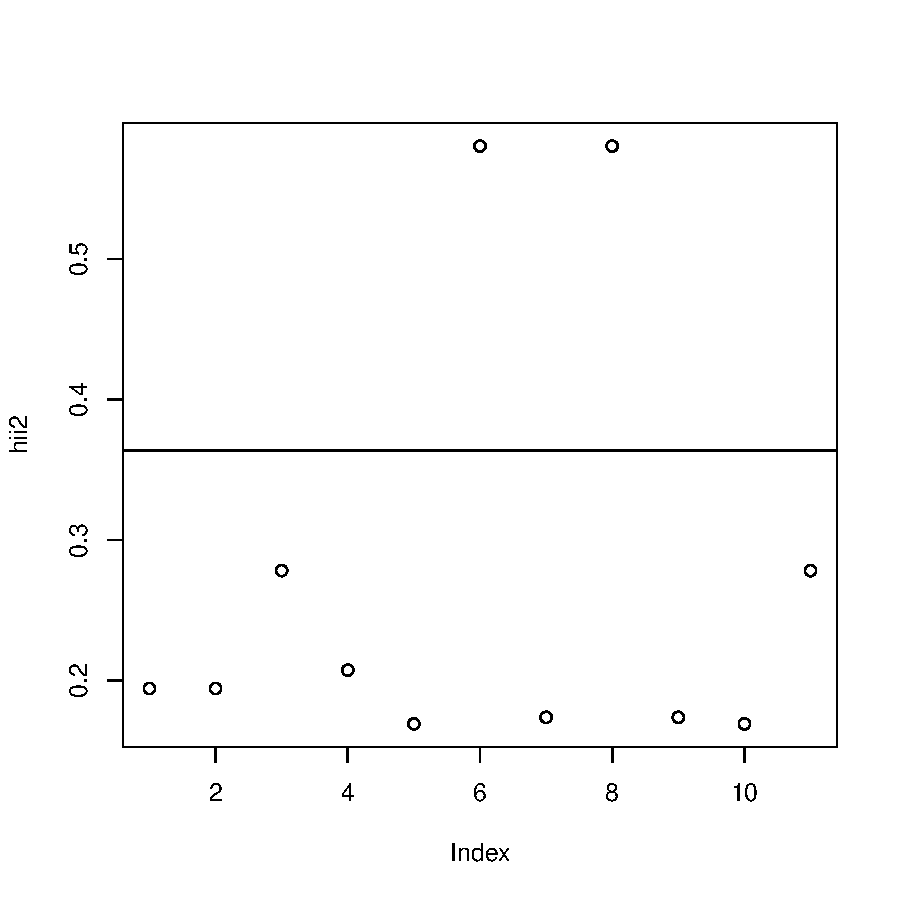
\includegraphics{HW6-017}
\end{figure}
The above plot shows that there are 2 observations that lie out of the cutoff line. From inf2.1 vector these observation numbers are 6 and 8.
\clearpage

Plot of Cook's distance values:
\begin{figure}[H]
\begin{Schunk}
\begin{Sinput}
> cutoff.cd2<-1
> plot(cd2)
> abline(h=cutoff.cd2)
\end{Sinput}
\end{Schunk}
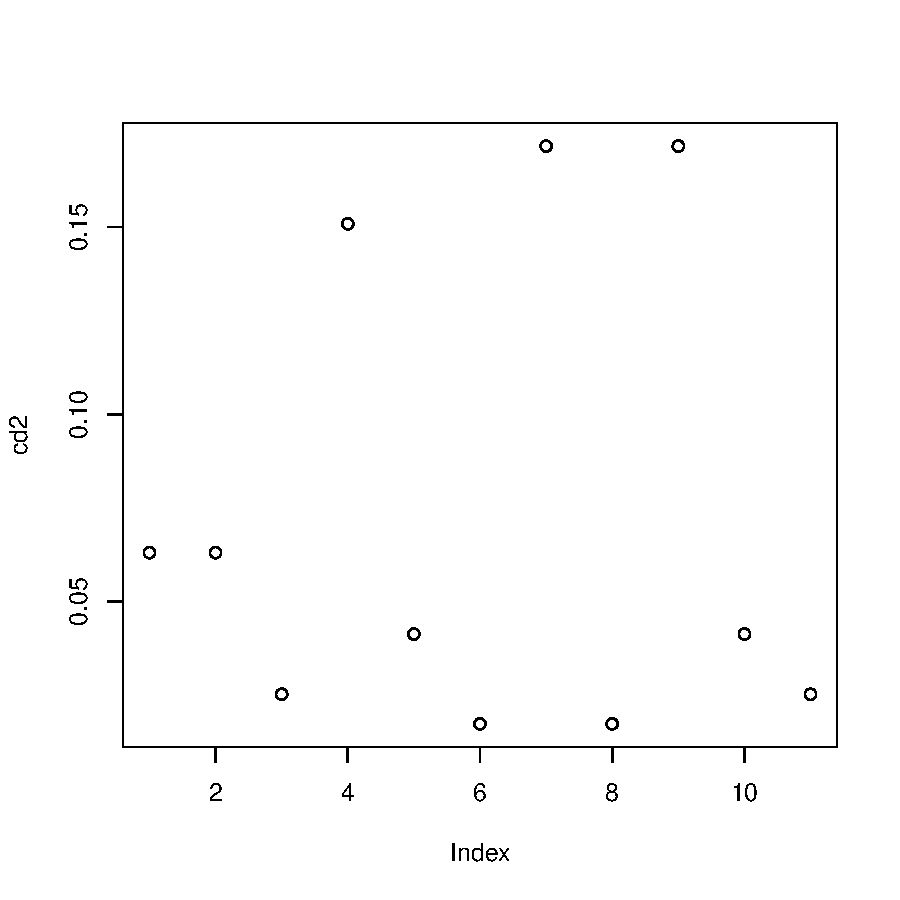
\includegraphics{HW6-018}
\end{figure}
The cutoff line is out of the bounds in this plot.

Thus observations 6 and 8 are influential points from the leverage criterion while the Cook's distance criterion does not give any influential point.

\clearpage

\item Analysis of $(x_3, y_3)$ within the linear model framework:\\
Scatter plot of $(x_3, y_3)$ along the fitted line is given as:
\begin{figure}[H]
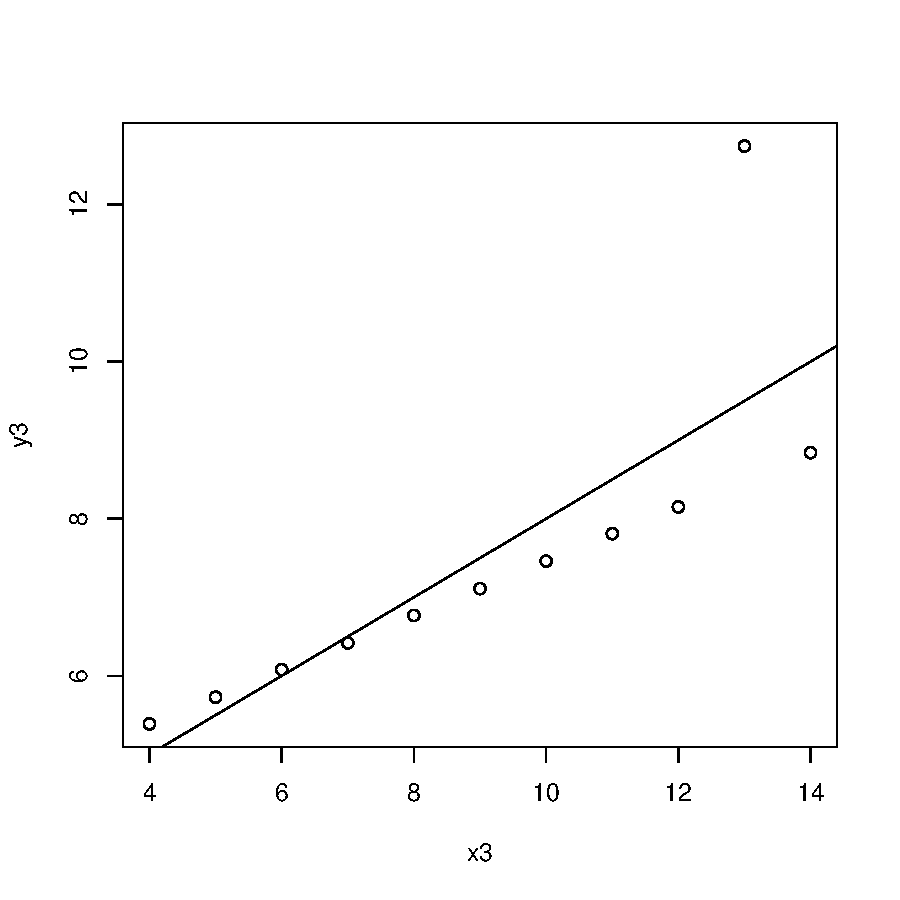
\includegraphics{HW6-019}
\end{figure}
The scatter plot shows that there is one outlier that is affecting the regression line. Otherwise the relationship seems to be linear and hence no transformations required. Calculating the studentized residuals and doing the test for identifying outliers confirms this as follows:
\begin{Schunk}
\begin{Sinput}
> rst3<-rstudent(fit3)
\end{Sinput}
\end{Schunk}
The following R code compares the values of the studentized residuals with the $\left(1-\dfrac{\alpha}{2}\right)$ quantile values of the t-distribution.

\begin{Schunk}
\begin{Sinput}
> # observation numbers of the outliers
> out3<-rep(0,length(x3))
> rst3<-rstudent(fit3)
> j=1
> for (i in 1:length(x3)){
+   if (rst3[i]>qt((1-(alpha/(2*length(x3)))),(n-p-1))){
+     out3[j]<-i
+     j<-j+1
+   }
+ }
> out3
\end{Sinput}
\begin{Soutput}
 [1] 3 0 0 0 0 0 0 0 0 0 0
\end{Soutput}
\end{Schunk}

Plotting the studentized residuals:
\begin{figure}[H]
\begin{Schunk}
\begin{Sinput}
> plot(rst3)
> cutoff<-qt(.975,df=n-p-1)
> abline(h=cutoff)
> abline(h=-cutoff)
\end{Sinput}
\end{Schunk}
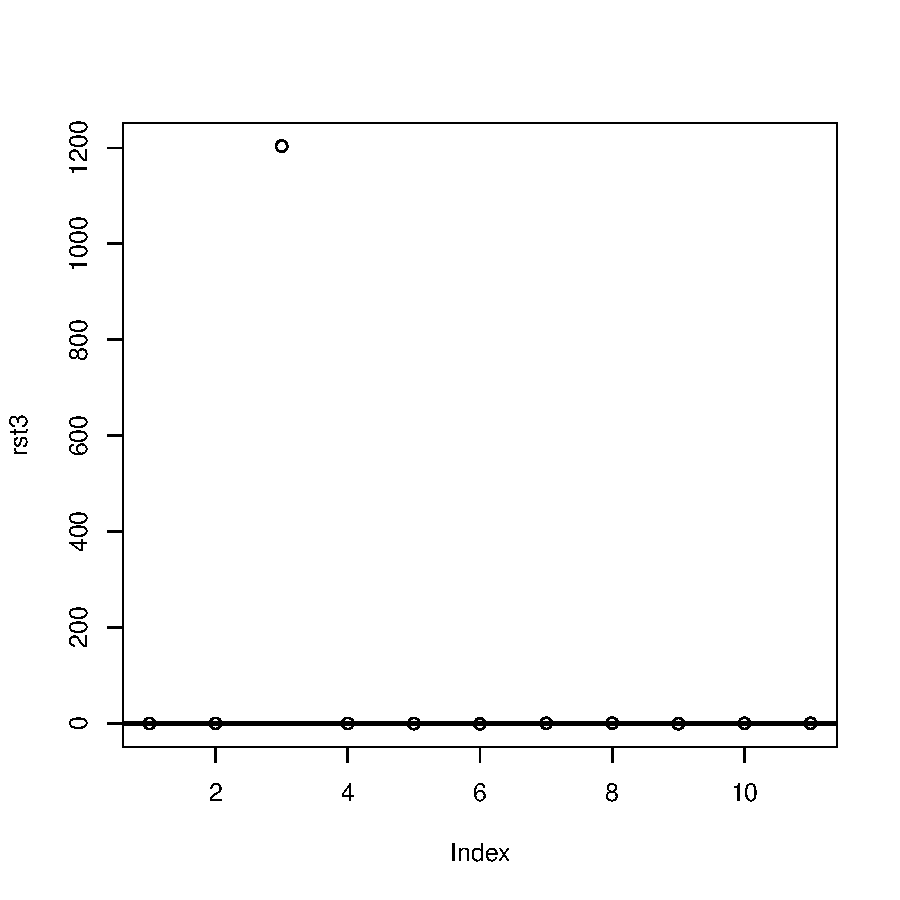
\includegraphics{HW6-022}
\end{figure}
\clearpage

Thus we see that observation 3 is an outlier. Again influential points were found using the leverage and Cook's distance criteria as follows:

\begin{Schunk}
\begin{Sinput}
> hii3<-hatvalues(fit3)
> cd3<-cooks.distance(fit3)
> inf3.1<-rep(0,length(x3))
> inf3.2<-rep(0,length(x3))
> j=1
> for (i in 1:length(x3)){
+   if (hii3[i]>(2*p/n)){
+     inf3.1[j]<-i
+     j<-j+1
+   }
+ }
> j=1
> for (i in 1:length(x2)){
+   if (cd3[i]>1){
+     inf3.2[j]<-i
+     j<-j+1
+   }
+ }
> inf3.1
\end{Sinput}
\begin{Soutput}
 [1] 0 0 0 0 0 0 0 0 0 0 0
\end{Soutput}
\begin{Sinput}
> inf3.2
\end{Sinput}
\begin{Soutput}
 [1] 3 0 0 0 0 0 0 0 0 0 0
\end{Soutput}
\end{Schunk}
\clearpage

Plotting the  diagonal hat values:
\begin{figure}[H]
\begin{Schunk}
\begin{Sinput}
> cutoff.h<-2*p/n
> plot(hii3)
> abline(h=cutoff.h)
\end{Sinput}
\end{Schunk}
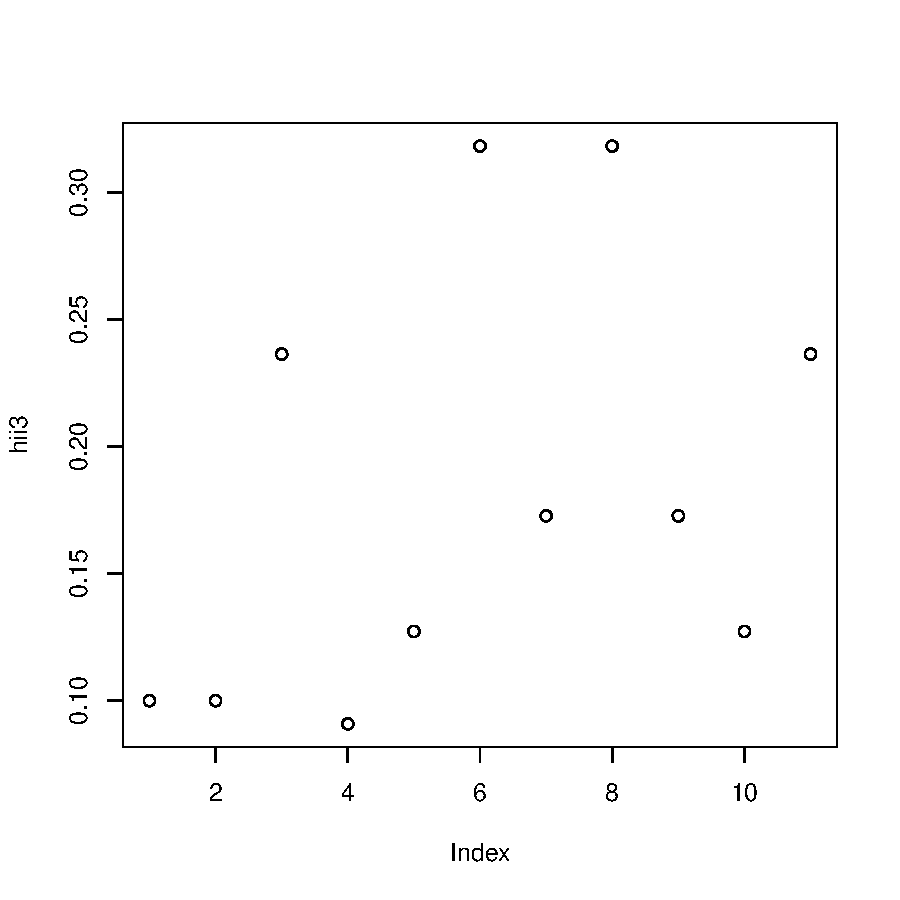
\includegraphics{HW6-024}
\end{figure}
The above plot shows that the cutoff lines are out of bounds.
\clearpage

Plot of Cook's distance values:
\begin{figure}[H]
\begin{Schunk}
\begin{Sinput}
> cutoff.cd3<-1
> plot(cd3)
> abline(h=cutoff.cd3)
\end{Sinput}
\end{Schunk}
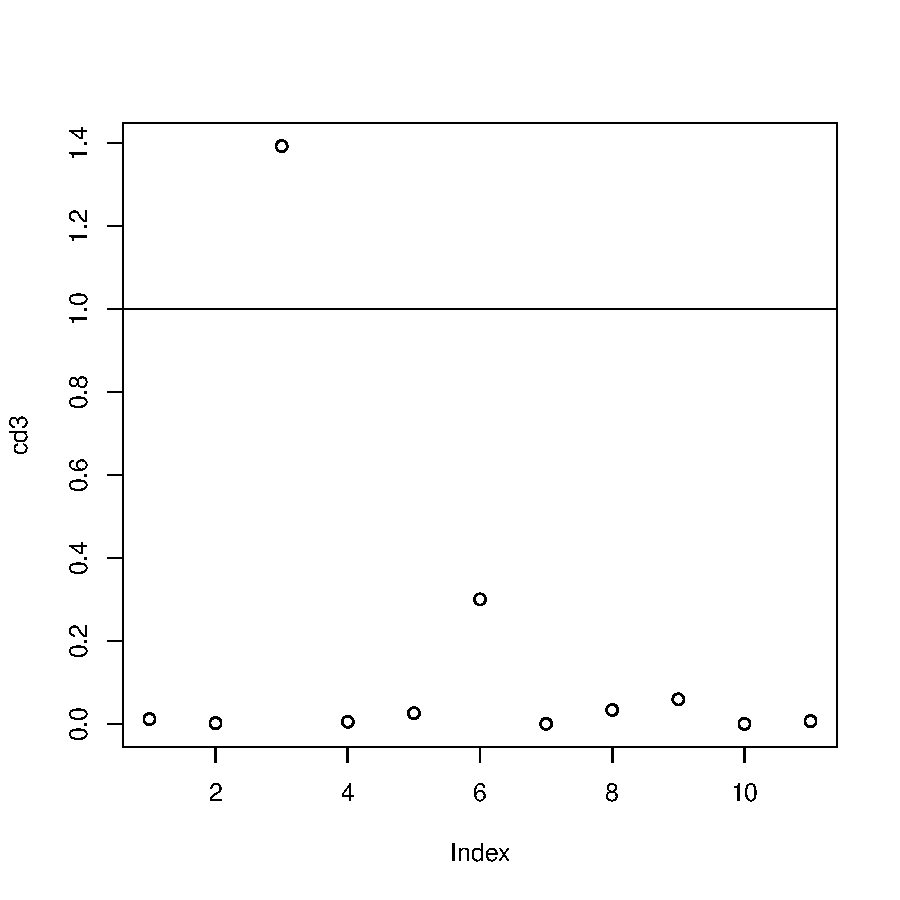
\includegraphics{HW6-025}
\end{figure}
The above plot shows that there is one observation that lies out of the cutoff line. From inf3.2 vector this is observation number 3.

Thus there are no influential points according to the leverage criterion while the Cook's distance criterion gives observation 3 as an influential point.

Since according to Cook's distance, the outlier observation number 3 is also influential it may be wise to drop it.   

Removing this outlier and fitting the model again we get

\begin{figure}[H]
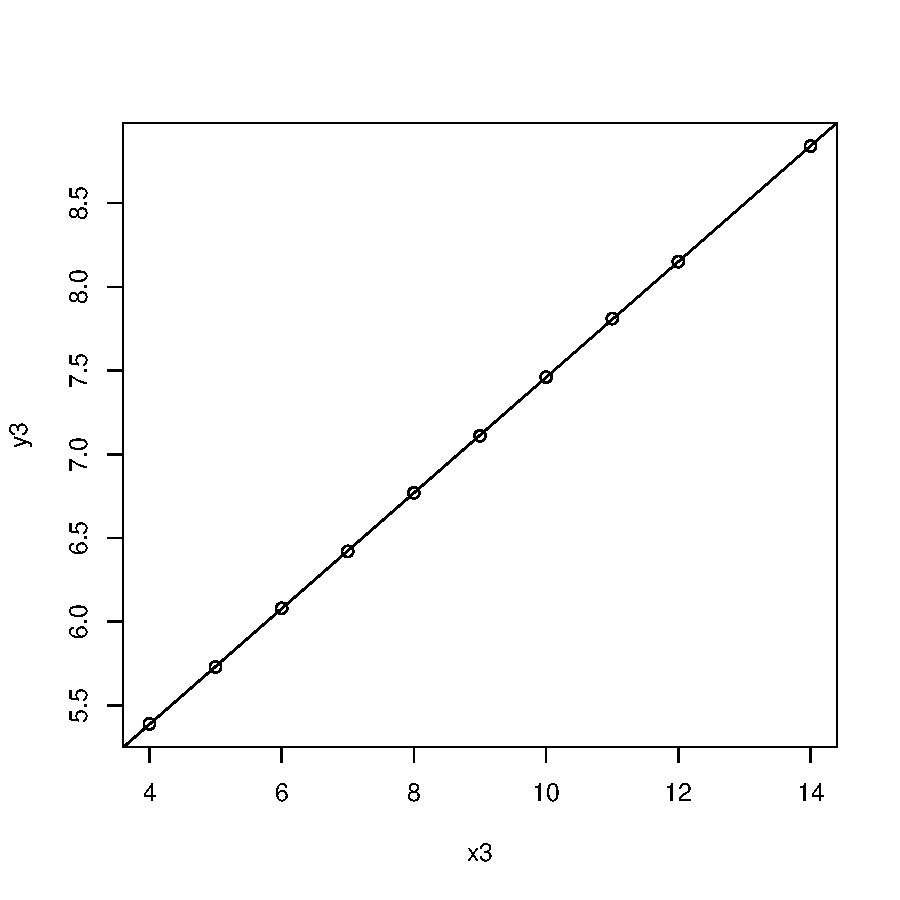
\includegraphics{HW6-026}
\end{figure}

which looks like a perfect fit. The new estimated parameters are:
\begin{Schunk}
\begin{Soutput}
(Intercept)          x3 
  4.0056494   0.3453896 
\end{Soutput}
\end{Schunk}
\clearpage

\item Analysis of $(x_4, y_4)$ within the linear model framework:\\
Scatter plot of $(x_4, y_4)$ along the fitted line is given as:
\begin{figure}[H]
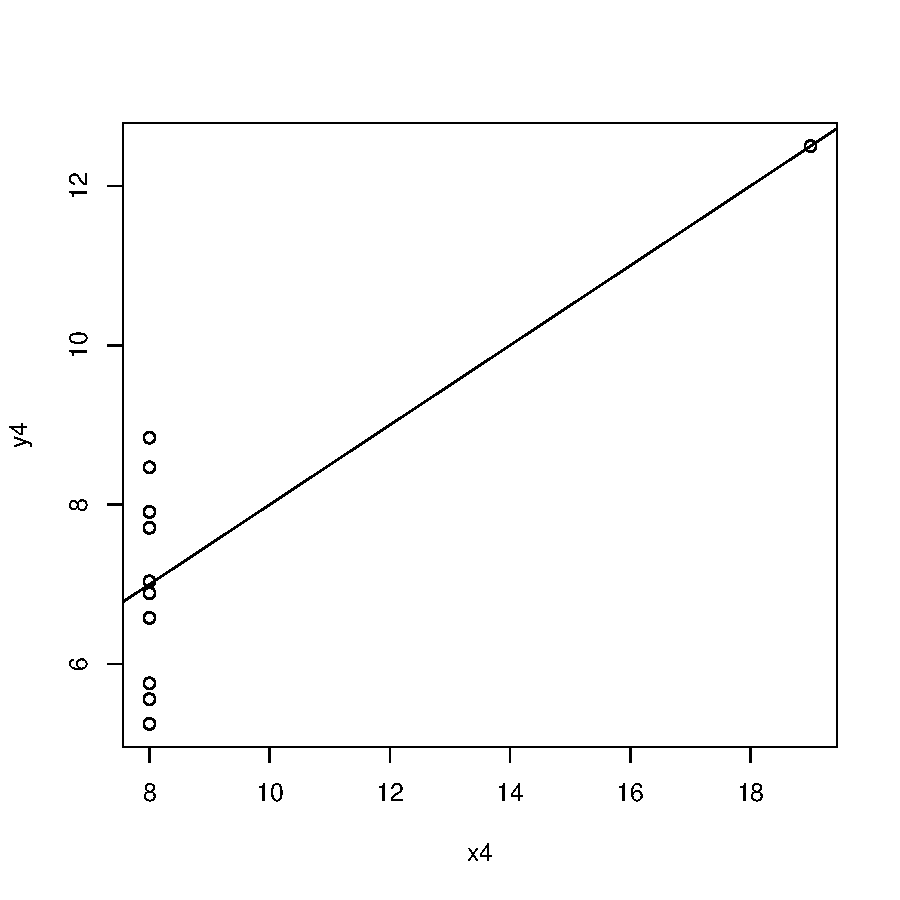
\includegraphics{HW6-028}
\end{figure}
In this case, the scatter plot clearly shows that there is an outlier. However it seems that the experimenter who took the data measured the response many times on one value of the predictor and only once for another value of the predictor. The scatter in different values of response may be a result of instrumental errors. The relationship between x and y still seems to be linear with some slope and there is no reason to neglect the outlier.\\
\clearpage
The residual plot is given as
\begin{figure}[H]
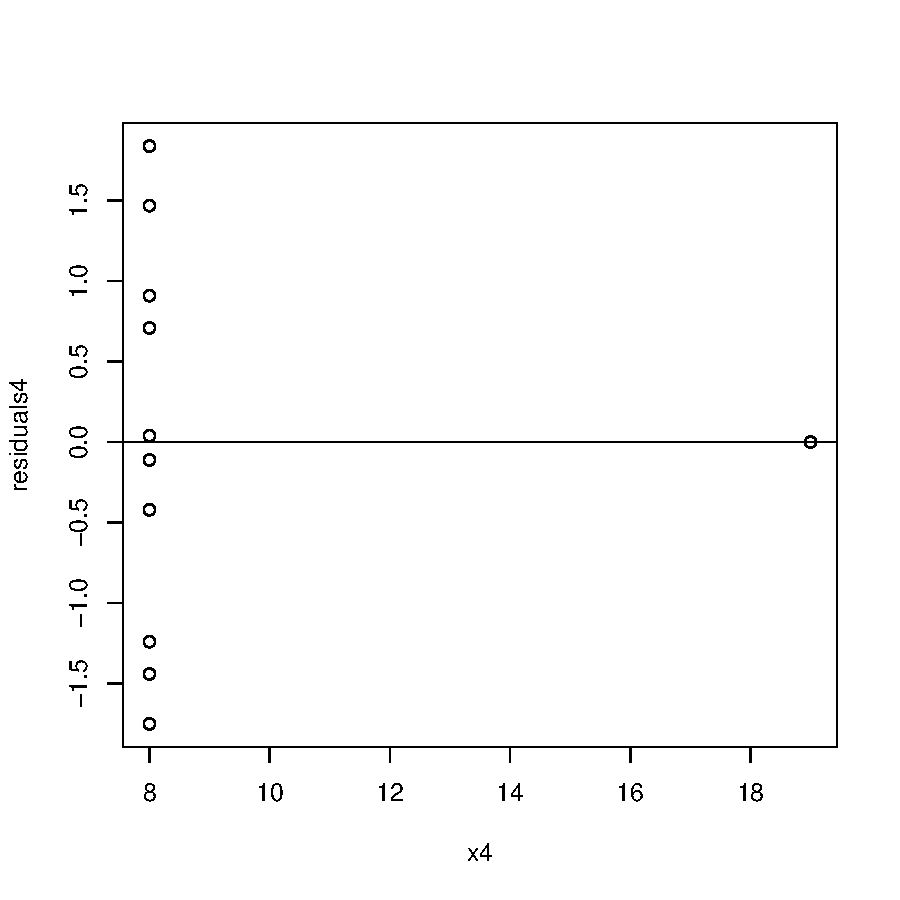
\includegraphics{HW6-029}
\end{figure}
The above residual plot shows that the residuals are uniformly distributed around 0. Thus our assumption of homoscedascity is verified. Further there does not seem any positive or negative correlation between successive values of residuals which verifies the assumption of independence. It may appear at the first glance that there is a non-linear trend. However this is merely an artifact since we only have two data points effectively corresponding to two different predictor values. \\

\end{itemize}

\item Predicting $E(y)$ and $95\%$ prediction intervals at $x=13$ for all the fitted models:

\begin{itemize}
\item For the first model, the predicted value of y at x=13 along with the 95\% confidence interval are given as
\begin{Schunk}
\begin{Sinput}
> newdata1=data.frame(x1=13)
> predict(fit1, newdata1, interval="predict")
\end{Sinput}
\begin{Soutput}
       fit      lwr      upr
1 9.501273 6.390801 12.61174
\end{Soutput}
\end{Schunk}

The modeling assumptions for the fitted model are satisfied in this case and so 95\% prediction intervals can be trusted.

\item For the second model, the predicted value of y at x=13 along with the 95\% confidence interval are given as
\begin{Schunk}
\begin{Sinput}
> newdata2=data.frame(x2=13)
> predict(fit2.2, newdata2, interval="predict")
\end{Sinput}
\begin{Soutput}
       fit      lwr     upr
1 8.740629 8.736269 8.74499
\end{Soutput}
\end{Schunk}

The assumption of homoscedascity from the residual plot does not seem to hold good even for the polynomial model and so the 95\% prediction interval can't be trusted.

\item For the third model, the predicted value of y at x=13 along with the 95\% confidence interval are given as
\begin{Schunk}
\begin{Sinput}
> newdata3=data.frame(x3=13)
> predict(fit3.2, newdata3, interval="predict")
\end{Sinput}
\begin{Soutput}
       fit      lwr      upr
1 8.495714 8.487582 8.503846
\end{Soutput}
\end{Schunk}

The model fitted without the outlier looks very good and so 95\% prediction intervals based on this model can be trusted.

\item For the last model, the predicted value of y at x=13 along with the 95\% confidence interval are given as
\begin{Schunk}
\begin{Sinput}
> newdata4=data.frame(x4=13)
> predict(fit4, newdata4, interval="predict")
\end{Sinput}
\begin{Soutput}
       fit      lwr      upr
1 9.500545 6.392357 12.60873
\end{Soutput}
\end{Schunk}
The 95\% prediction intervals based on this model is solely based on the data point corresponding to the 2nd value of the predictor. Already the interval is very wide pointing to a high uncertainity. Thus it can be trusted but with a pinch of salt.
\end{itemize}
\en
\end{document}
